%LTeX: language=pt-br
% !TeX root = Apostila_IM381.tex

\cleardoublepage
\section{Problema de condução de calor}
\label{sec:conducao}

    Agora que vimos como o MEF funciona para modelos unidimensionais, vamos passar para o caso bidimensional mais simples: o problema de condução de calor. Os procedimentos usados aqui são os mesmos que para os casos anteriores.

    \subsection{Equação diferencial da condução de calor}

        Considere um domínio $\Omega$ sujeito a uma geração interna de calor $p(x,y)$ (Figura \ref{fig:dominio_calor}). O domínio possui uma condutividade térmica constante de $k$ (se ele for variável, não há alterações significativas na formulação). Em um determinado ponto $\mathbf{x} = \left[x, y\right]^T$ do domínio, o fluxo de calor por área é dada pela lei de Fourier:

        \begin{figure}[h!]
            \centering
            
\includegraphics[scale=1.5]{Figures/7-Calor/Dominio.pdf}
            \caption{Domínio de um problema de condução de calor}
            \label{fig:dominio_calor}
        \end{figure}

        \begin{equation}
            \mathbf{q} = 
            \begin{Bmatrix}
                q_x \\
                q_y \\
            \end{Bmatrix} =
            -k \nabla T = -k 
            \begin{Bmatrix}
                \frac{\partial T}{\partial x} \\
                \frac{\partial T}{\partial y} \\
            \end{Bmatrix}
        \end{equation}

        \noindent no qual o sinal de menos indica que o fluxo de calor segue o sentido de maiores temperaturas para menores.

        Fazendo um balanço de energia em um volume de controle infinitesimal do domínio, considerando temperatura crescente com $x$ e $y$ (Figura \ref{fig:calor_infinitesimal}):

        \begin{figure}[h!]
            \centering
            
\includegraphics[scale=1.4]{Figures/7-Calor/Infinitesimal.pdf}
            \caption{Volume de controle infinitesimal para o balanço de energia do problema de condução}
            \label{fig:calor_infinitesimal}
        \end{figure}

        \begin{equation*}
            q_x dy + q_y dx - q_{x+dx} dy - q_{y+dy} dx + p(x,y) dx dy = 0
        \end{equation*}

        \begin{equation*}
            -k\frac{\partial T}{\partial x} dy 
            -k\frac{\partial T}{\partial y} dx 
            + k\frac{\partial T}{\partial x} dy + \frac{\partial}{\partial x}\left(k\frac{\partial T}{\partial x}\right) dx dy 
            + k\frac{\partial T}{\partial y} dx + \frac{\partial}{\partial y}\left(k\frac{\partial T}{\partial y}\right) dy dx 
            + p(x,y) dx dy = 0
        \end{equation*}

        Portanto, a equação diferencial da condução de calor fica:

        \begin{equation}
            k\frac{\partial^2 T}{\partial x^2}
            +k\frac{\partial^2 T}{\partial y^2}
             = -p(x,y)
        \end{equation}

        Que pode ser escrita com os operadores de divergente ($\nabla \cdot \square$), gradiente ($\nabla \square$) ou o laplaciano, definido como o divergente do gradiente ($\Delta = \nabla \cdot \nabla \square$):

        \begin{equation}
            k \Delta T = k \nabla \cdot \left(\nabla T\right)
             = -p(x,y)
        \end{equation}

        Esta equação também requer condições de contorno ao longo de sua volta completa. Elas podem ser também condições de contorno de Dirichlet, com temperatura imposta em alguma parte de sua superfície:

        \begin{equation}
            T(\mathbf{x}) = T_0 \quad, x \in \Gamma_1 \subset \partial \Omega
        \end{equation}

        \noindent no qual $\Gamma_1$ é alguma superfície no entorno do domínio. O símbolo $\partial \Omega$ representa o fecho (as bordas) do domínio $\Omega$.

        Também pode haver condições de Neumann, representando fluxos de calor impostos na superfície. No caso de condições de contorno, o que importa é o fluxo normal ao fecho do domínio, visto que a tangente é regida pela equação diferencial:

        \begin{equation}
            k\frac{\partial T}{\partial \mathbf{n}} = q_0 \quad, x \in \Gamma_2 \subset \partial \Omega
        \end{equation}

        \noindent no qual $\Gamma_2$ representa uma outra superfície do domínio. O vetor $\mathbf{n}$ é o vetor normal à superfície.

        A condição de contorno mais comum é a de \textbf{superfície adiabática}, ou seja, na qual não há perda de calor para o ambiente. Neste caso, na condição de contorno de Neumann apresentada acima temos $q_0 = 0$.

    \subsection{Forma fraca e aproximação da solução}

        A equação diferencial da forma que obtivemos está na forma forte. Para passarmos para a forma fraca, realizamos o mesmo procedimento que fizemos anteriormente. Inserindo uma função peso $w(x,y)$ no sistema:

        \begin{equation}
            \int_\Omega w(x,y) k \nabla \cdot \left(\nabla T(x,y)\right) dA + \int_\Omega w(x,y) p(x,y) dA = 0 \quad, \forall w(x,y) \in W
            \label{eq:calor_fraca_part1}
        \end{equation}

        Para simplificar as notações, vamos suprimir as dependências por $x$ e $y$. Considere a integral abaixo, podemos utilizar a regra do produto no divergente:

        \begin{equation}
            \int_\Omega \nabla \cdot \left( w\nabla T \right) dA  = 
            \int_\Omega w \nabla \cdot \left(\nabla T\right) dA + 
            \int_\Omega \nabla w^T \nabla T  dA
        \end{equation}

        O primeiro termo pode ser substituído usando o teorema do divergente:

        \begin{equation}
            \int_\Omega \nabla \cdot \left( w\nabla T \right) dA  = 
            \int_{\partial \Omega} w\nabla T \cdot \mathbf{n} d\Gamma
        \end{equation}

        Portanto, temos a seguinte relação ao juntarmos as duas equações:

        \begin{equation}
            \int_\Omega w \nabla \cdot \left(\nabla T\right) dA = 
            \int_{\partial \Omega} w\nabla T \cdot \mathbf{n} d\Gamma -
            \int_\Omega \nabla w \nabla T  dA
        \end{equation}

        Podemos voltar, portanto, para a Eq. \eqref{eq:calor_fraca_part1}:

        \begin{equation*}
            \int_\Omega w k \nabla \cdot \left(\nabla T\right) dA + \int_\Omega w p dA = 0
        \end{equation*}

        \begin{equation*}
            \int_{\partial \Omega} k w\nabla T \cdot \mathbf{n} d\Gamma -
            \int_\Omega k \nabla w^T \nabla T  dA + \int_\Omega w p dA = 0
        \end{equation*}

        \begin{equation}
            \int_\Omega k \nabla w^T \nabla T  dA = 
            \int_{\partial \Omega} k w\nabla T \cdot \mathbf{n} d\Gamma
             + \int_\Omega w p dA \quad ,\forall w \in W
        \end{equation}

        Esta equação representa a forma fraca do problema de condução de calor. Note as similaridades, embora de forma mais complexa, com as equações anteriores. O termo à esquerda da igualdade tem um operador bidirecional entre a função peso e a função incógnita. À direita da igualdade, temos um termo representando as condições de contorno nas interfaces do domínio, e um termo de geração interna, similar ao das forças de campo dos problemas de barra e de viga.

        O próximo passo para a solução é definir um espaço de funções candidatas $T^h(x,y) \in V^h \subset V$ e de funções ponderadoras $w^h(x,y) \in W^h \subset W$. Com o método dos resíduos ponderados, chegamos a uma forma fraca aproximada similar:

        \begin{equation}
            \int_\Omega k \nabla {w^h}^T \nabla T^h  dA = 
            \int_{\partial \Omega} k w^h\nabla T^h \cdot \mathbf{n} d\Gamma
             + \int_\Omega w^h p dA \quad ,\forall w \in W^h
             \label{eq:calor_fraca_aprox}
        \end{equation}


    \subsection{Método de Galerkin}

        Com o método de Galekin, usamos $W^h = V^h$. Portanto, o que nos falta agora é definir quem serão as funções de forma usadas aqui. Já será usada a construção teórica de subdividir o domínio em elementos, estes definidos por funções de forma em suas próprias coordenadas locais. Quais são exatamente essas funções e os domínios, veremos em seguida.

        Considere um elemento cujas coordenadas locais são dadas por $\bar{x}$ e $\bar{y}$. A temperatura e a função teste aproximada no interior desse elemento são interpoladas pelas funções de forma:

        \begin{equation}
            T^h(\bar{x},\bar{y}) = \sum_i N(\bar{x},\bar{y}) a_i = \mathbf{N} \mathbf{a}_e
        \end{equation}

        \begin{equation}
            w^h(\bar{x},\bar{y}) = \sum_i N(\bar{x},\bar{y}) b_i = \mathbf{N} \mathbf{b}_e
        \end{equation}

        No elemento, com um domínio $\Omega_e \subset \Omega$, com uma parte da interface $\Gamma_e \subset \partial \Omega_e$:

        \begin{equation}
            \int_{\Omega_e} k \nabla {w^h}^T \nabla T^h  dA = 
            \int_{\Gamma_e} k w^h\nabla T^h \cdot \mathbf{n} d\Gamma
             + \int_{\Omega_e} w^h p dA \quad ,\forall w \in W^h
             \label{eq:calor_fraca_elemento}
        \end{equation}

        O termo de derivada na primeira integral é o seguinte:

        \begin{equation*}
            \nabla T^h =  
            \begin{Bmatrix}
                \frac{\partial T^h}{\partial x}\\
                \frac{\partial T^h}{\partial y}
            \end{Bmatrix} =
            \begin{Bmatrix}
                \frac{\partial \mathbf{N} \mathbf{a}_e}{\partial x}\\
                \frac{\partial \mathbf{N} \mathbf{a}_e}{\partial y}
            \end{Bmatrix}
        \end{equation*}

        Para transformar este último termo em algo do tipo $\mathbf{B} \mathbf{a}_e$:

        \begin{equation}
            \nabla T^h =  
            \begin{Bmatrix}
                \frac{\partial \mathbf{N} \mathbf{a}}{\partial x}\\
                \frac{\partial \mathbf{N} \mathbf{a}}{\partial y}
            \end{Bmatrix} =
            \begin{bmatrix}
                \frac{\partial \mathbf{N}_1}{\partial x} & \frac{\partial \mathbf{N}_2}{\partial x} & \cdots & \frac{\partial \mathbf{N}_n}{\partial x}\\
                \frac{\partial \mathbf{N}_1}{\partial y} & \frac{\partial \mathbf{N}_2}{\partial y} & \cdots & \frac{\partial \mathbf{N}_n}{\partial y}\\
            \end{bmatrix}
            \begin{Bmatrix}
                a_1\\
                a_2\\
                \vdots\\
                a_n
            \end{Bmatrix}
            = 
            \mathbf{B}
            \mathbf{a}_e
            \label{eq:calor_B}
        \end{equation}


        Analogamente:

        \begin{equation*}
            \nabla w^h =  
            \begin{bmatrix}
                \frac{\partial \mathbf{N}_1}{\partial x} & \frac{\partial \mathbf{N}_2}{\partial x} & \cdots & \frac{\partial \mathbf{N}_n}{\partial x}\\
                \frac{\partial \mathbf{N}_1}{\partial y} & \frac{\partial \mathbf{N}_2}{\partial y} & \cdots & \frac{\partial \mathbf{N}_n}{\partial y}\\
            \end{bmatrix}
            \begin{Bmatrix}
                b_1\\
                b_2\\
                \vdots\\
                b_n
            \end{Bmatrix}
            = 
            \mathbf{B}
            \mathbf{b}_e
        \end{equation*}
        
        Finalmente, voltando à primeira integral da Eq. \eqref{eq:calor_fraca_elemento}:

        \begin{equation*}
            \int_{\Omega_e} k \nabla {w^h}^T \nabla T^h  dA = \mathbf{b}_e^T  k\int_{\Omega_e} \mathbf{B}^T \mathbf{B} dA \;\mathbf{a}_e
        \end{equation*}

        No caso de condução de calor, podemos considerar que:

        \begin{equation}
            \mathbf{D} = 
            \begin{bmatrix}
                k & 0\\
                0 & k
            \end{bmatrix}
        \end{equation}

        Para chegarmos à forma geral:

        \begin{equation*}
            \mathbf{b}_e^T  \int_{\Omega_e} \mathbf{B}^T \mathbf{D} \mathbf{B} dA \; \mathbf{a}_e
        \end{equation*}

        Similarmente para os termos de força:

        \begin{equation}
            \int_{\Gamma_e} k w^h\nabla T^h \cdot \mathbf{n} d\Gamma = -
            \mathbf{b}_e^T  \int_{\Gamma_e} \mathbf{N}^T \left(\mathbf{q} \cdot \mathbf{n}\right) d\Gamma
        \end{equation}

        \begin{equation}
            \int_{\Omega_e} w^h p dA =
            \mathbf{b}_e^T  \int_{\Omega_e} \mathbf{N}^T p(x,y) dA
        \end{equation}

        Portanto, substituindo estes na Eq. \eqref{eq:calor_fraca_elemento}, e sabendo que esta equação deve ser válida para qualquer $\mathbf{b}$, chegamos ao sistema:


        \begin{equation}
            \int_{\Omega_e} \mathbf{B}^T \mathbf{D} \mathbf{B} dA \; \mathbf{a}_e = 
            \int_{\Gamma_e} \mathbf{N}^T \left(\mathbf{q} \cdot \mathbf{n}\right) d\Gamma +
            \int_{\Omega_e} \mathbf{N}^T p(x,y) dA
            \label{eq:calor_eq_elemento}
        \end{equation}


        \begin{equation}
            \mathbf{K}_e \mathbf{a}_e = \mathbf{f}_e
        \end{equation}

        Da mesma forma como anteriormente, realizamos a montagem do sistema global a partir das matrizes elementares. Resolvemos o sistema global:

        \begin{equation}
            \mathbf{K} \mathbf{a} = \mathbf{f},
        \end{equation}

        \noindent que nos retorna os coeficientes que usamos para reconstruir o campo de temperatura do domínio, interpolando em cada elemento.

        Com os coeficientes, podemos calcular também os fluxos de calor por unidade de área:

        \begin{equation}
            \mathbf{q}(\bar{x},\bar{y}) = - k \nabla T^h = - \mathbf{D} \mathbf{B} \mathbf{a}_e
            \label{eq:fluxo_reconstruido}
        \end{equation}


    \subsection{Elemento triangular regular}
    \label{sec:elemento_triangular}

        O elemento com a formulação mais simples, embora em alguns aspectos seja relativamente complexo, é o triângulo. Considere o elemento triangular da Figura \ref{fig:element_triangulo}, as coordenadas locais em elementos deste tipo são normalmente definidas pelas três áreas ($A_1$, $A_2$ e $A_3$) definidas pelos três vértices e o ponto interno.

        \begin{figure}[h!]
            \centering
            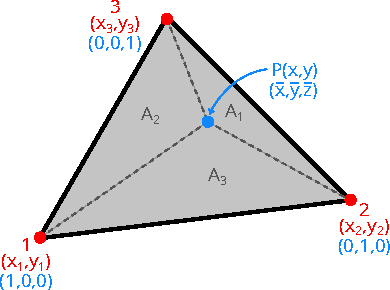
\includegraphics[scale=1.4]{Figures/7-Calor/Triangulo.pdf}
            \caption{Elemento triangular definido pelas coordenadas locais}
            \label{fig:element_triangulo}
        \end{figure}

        As coordenadas locais $\bar{x}$, $\bar{y}$ e $\bar{z}$ (não confunda a nomenclatura aqui como um sistema em três dimensões) podem ser definidas como:

        \begin{equation}
            \bar{x} = \frac{A_1}{A} \quad \bar{y} = \frac{A_2}{A} \quad \bar{z} = \frac{A_3}{A}
        \end{equation}

        \noindent no qual $A = A_1 + A_2 + A_3$. Portanto, $\bar{x} + \bar{y} + \bar{z} = 1$ e, consequentemente:

        \begin{equation}
            \bar{z} = 1 - \bar{x} - \bar{y}
        \end{equation}

        As coordenadas globais em um ponto qualquer é dado por:

        \begin{equation}
            x = \bar{x} x_1 + \bar{y} x_2 + \bar{z} x_3 = \sum_i N_i x_i
        \end{equation}

        \begin{equation}
            y = \bar{x} y_1 + \bar{y} y_2 + \bar{z} y_3 = \sum_i N_i y_i
        \end{equation}

        \begin{equation}
            \mathbf{x} = 
            \begin{Bmatrix}
                x\\
                y
            \end{Bmatrix} = 
            \mathbf{N} \mathbf{x_n}
        \end{equation}

        \noindent no qual $\mathbf{x_n}^T = 
        \begin{bmatrix}
                x_1 &
                y_1 &
                x_2 &
                y_2 &
                x_3 &
                y_3 &
            \end{bmatrix}$ e $ 
            \mathbf{N} = 
            \begin{bmatrix}
                \bar{x} &
                \bar{x} &
                \bar{y} &
                \bar{y} &
                1 - \bar{x} - \bar{y} &
                1 - \bar{x} - \bar{y}
            \end{bmatrix}$. Isto é, $N_1(\bar{x},\bar{y}) = \bar{x}$, $N_2(\bar{x},\bar{y}) = \bar{y}$ e $N_3(\bar{x},\bar{y}) = 1 - \bar{x} - \bar{y}$. Essas funções de forma têm a mesma propriedade dos polinômios de Lagrange, isto é, quando usadas para interpolar as temperaturas, os coeficientes do sistema representam as temperaturas nos nós correspondentes a cada uma dessas funções de forma. Note que neste caso, no entanto, não há a propriedade de superconvergência, então as temperaturas nodais não serão exatas.

        As derivadas das coordenadas globais em relação a cada coordenada local é dada por:

        \begin{equation*}
            \frac{\partial x}{\partial \bar{x}} = x_1 - x_3 \quad \frac{\partial x}{\partial \bar{y}} = x_2 - x_3
            \quad \frac{\partial y}{\partial \bar{x}} = y_1 - y_3 \quad \frac{\partial y}{\partial \bar{y}} = y_2 - y_3
        \end{equation*}

        Podemos definir uma matriz chamada \textbf{Jacobiano}:

        \begin{equation}
            \mathbf{J} = 
            \begin{bmatrix}
                 \frac{\partial x}{\partial \bar{x}} &  \frac{\partial y}{\partial \bar{x}}\\
                 \frac{\partial x}{\partial \bar{y}} &  \frac{\partial y}{\partial \bar{y}}
            \end{bmatrix}
        \end{equation}

        \noindent cujo determinante aqui é dado por:

        \begin{equation}
            \det \mathbf{J} = \left(x_1 - x_3\right)\left(y_2 - y_3\right) - \left(x_2 - x_3\right)\left(y_1 - y_3\right) = 2A
        \end{equation}

        A derivada de uma função qualquer $f(x,y)$ em relação às coordenadas locais e às globais podem ser relacionadas pela regra da cadeia:

        \begin{equation*}
            \frac{\partial f}{\partial \bar{x}} = 
            \frac{\partial f}{\partial x} \frac{\partial x}{\partial \bar{x}} + 
            \frac{\partial f}{\partial y} \frac{\partial y}{\partial \bar{x}} =
            \begin{bmatrix}
                \frac{\partial x}{\partial \bar{x}} &
                \frac{\partial y}{\partial \bar{x}}
            \end{bmatrix}
            \begin{Bmatrix}
                \frac{\partial f}{\partial x} \\
                \frac{\partial f}{\partial y}
            \end{Bmatrix}
        \end{equation*}

        \begin{equation*}
            \frac{\partial f}{\partial \bar{y}} = 
            \frac{\partial f}{\partial x} \frac{\partial x}{\partial \bar{y}} + 
            \frac{\partial f}{\partial y} \frac{\partial y}{\partial \bar{y}} =
            \begin{bmatrix}
                \frac{\partial x}{\partial \bar{y}} &
                \frac{\partial y}{\partial \bar{y}}
            \end{bmatrix}
            \begin{Bmatrix}
                \frac{\partial f}{\partial x} \\
                \frac{\partial f}{\partial y}
            \end{Bmatrix}
        \end{equation*}

        \begin{equation}
            \begin{Bmatrix}
                \frac{\partial f}{\partial \bar{x}} \\
                \frac{\partial f}{\partial \bar{y}}
            \end{Bmatrix} =
            \begin{bmatrix}
                \frac{\partial x}{\partial \bar{x}} & \frac{\partial y}{\partial \bar{x}}\\
                \frac{\partial x}{\partial \bar{y}} & \frac{\partial y}{\partial \bar{y}}
            \end{bmatrix}
            \begin{Bmatrix}
                \frac{\partial f}{\partial x} \\
                \frac{\partial f}{\partial y}
            \end{Bmatrix}
            = \mathbf{J}
            \begin{Bmatrix}
                \frac{\partial f}{\partial x} \\
                \frac{\partial f}{\partial y}
            \end{Bmatrix}
        \end{equation}
        

        \begin{equation}
            \begin{Bmatrix}
                \frac{\partial f}{\partial x} \\
                \frac{\partial f}{\partial y}
            \end{Bmatrix} = 
            \mathbf{J}^{-1}
            \begin{Bmatrix}
                \frac{\partial f}{\partial \bar{x}} \\
                \frac{\partial f}{\partial \bar{y}}
            \end{Bmatrix}
        \end{equation}

        No problema térmico, como verificamos anteriormente, precisamos das derivadas das funções de forma em relação às coordenadas globais. Elas podem ser obtidas desta forma:

        \begin{equation}
            \begin{Bmatrix}
                \frac{\partial N_1}{\partial x} \\
                \frac{\partial N_1}{\partial y}
            \end{Bmatrix} = 
            \mathbf{J}^{-1}
            \begin{Bmatrix}
                \frac{\partial N_1}{\partial \bar{x}} \\
                \frac{\partial N_1}{\partial \bar{y}}
            \end{Bmatrix} = 
            \mathbf{J}^{-1}
            \begin{Bmatrix}
                1 \\
                0
            \end{Bmatrix}
            \quad 
            \begin{Bmatrix}
                \frac{\partial N_2}{\partial x} \\
                \frac{\partial N_2}{\partial y}
            \end{Bmatrix} = 
            \mathbf{J}^{-1}
            \begin{Bmatrix}
                0 \\
                1
            \end{Bmatrix}
            \quad
            \begin{Bmatrix}
                \frac{\partial N_3}{\partial x} \\
                \frac{\partial N_3}{\partial y}
            \end{Bmatrix} = 
            \mathbf{J}^{-1}
            \begin{Bmatrix}
                -1 \\
                -1
            \end{Bmatrix}
        \end{equation}

        Resolvendo estes sistemas, obtemos as seguintes derivadas:

        \begin{equation*}
            \frac{\partial N_1}{\partial x} = \frac{y_2-y_3}{2A} \quad,
            \frac{\partial N_2}{\partial x} = \frac{y_3-y_1}{2A} \quad,
            \frac{\partial N_3}{\partial x} = \frac{y_1-y_2}{2A}
        \end{equation*}

        \begin{equation}
            \frac{\partial N_1}{\partial y} = \frac{x_3-x_2}{2A} \quad,
            \frac{\partial N_2}{\partial y} = \frac{x_1-x_3}{2A} \quad,
            \frac{\partial N_3}{\partial y} = \frac{x_2-x_1}{2A}
        \end{equation}

        Note que todos esses valores são \textbf{constantes}. Portanto, com eles, podemos montar a matriz $\mathbf{B}$ do problema de condução de calor, conforme a Eq. \eqref{eq:calor_B}.

        Finalmente, retornamos à integral da matriz de rigidez:

        \begin{equation*}
            \mathbf{K}_e = \int_{\Omega_e} \mathbf{B}^T \mathbf{D} \mathbf{B} dA
        \end{equation*}

        Em um domínio de ordem superior, a transformação de coordenadas é dada a partir da transformação dos dois integrandos ($dx$ e $dy$), nos integrandos ($d\bar{x}$ e $d\bar{y}$). O termo de derivada de um em relação ao outro é dado pelo \textbf{determinante do Jacobiano}. Finalmente, lembre-se que $\bar{x} + \bar{y} + \bar{z} = 1$. Portanto, o limite superior de integração para $\bar{y}$ deve ser $1-\bar{x}$, para não ultrapassar o limite.

        \begin{equation*}
            \int_{\Omega_e} \mathbf{B}^T \mathbf{D} \mathbf{B} dA = \int_{0}^{1} \int_{0}^{1-\bar{x}} \mathbf{B}^T \mathbf{D} \mathbf{B} \det \mathbf{J} d\bar{y} d\bar{x}
        \end{equation*}

        Todos os termos na integral são constantes, tanto em relação a $\bar{x}$ quanto a $\bar{y}$, portanto:


        \begin{equation}
            \mathbf{K}_e = \mathbf{B}^T \mathbf{D} \mathbf{B} \det \mathbf{J} \int_{0}^{1} \int_{0}^{1-\bar{x}}  d\bar{y} d\bar{x} = \frac{1}{2} \mathbf{B}^T \mathbf{D} \mathbf{B} \det \mathbf{J}
        \end{equation}


        O fluxo de calor dentro do elemento é dado pela Eq. \eqref{eq:fluxo_reconstruido}:

        \begin{equation*}
            \mathbf{q} = - k \nabla T^h = - \mathbf{D} \mathbf{B} \mathbf{a}_e
        \end{equation*}

        O fluxo de calor dentro de um elemento triangular será constante. Uma consequência é que na interface entre dois elementos, haverá uma descontinuidade no fluxo também.

        Sobre os termos de força, podemos integrá-los também. O termo da interface pode ser integrado como se fossem elementos unidimensionais, com sua variável sendo a parametrização desta superfície. O termo de geração de carga também pode ser integrada. Considere um caso com geração uniforme $p(x,y) = Q$:


        \begin{equation*}
            \int_{\Omega_e} \mathbf{N}^T Q dA = 
            Q \int_{0}^{1} \int_{0}^{1-\bar{x}} 
            \begin{Bmatrix}
                \bar{x}\\
                \bar{y}\\
                1-\bar{x}-\bar{y}
            \end{Bmatrix} \det \mathbf{J} d\bar{y} d\bar{x} = 
            Q \det \mathbf{J} \int_{0}^{1} \left.
            \begin{Bmatrix}
                \bar{x}\bar{y}\\
                \bar{y}^2/2\\
                \bar{y}-\bar{x}\bar{y}-\bar{y}^2/2
            \end{Bmatrix} \right|_{0}^{1-\bar{x}}  d\bar{x}
        \end{equation*}

        \begin{equation*}
             \int_{\Omega_e} \mathbf{N}^T Q dA = 2QA\int_{0}^{1} 
            \begin{Bmatrix}
                \bar{x}-\bar{x}^2\\
                1/2 - \bar{x} + \bar{x}^2/2\\
                1/2 - \bar{x} + \bar{x}^2/2
            \end{Bmatrix}  d\bar{x} = 
             2QA \left.
            \begin{Bmatrix}
                \bar{x}^2/2-\bar{x}^3/3\\
                \bar{x}/2 - \bar{x}^2/2 + \bar{x}^3/6\\
                \bar{x}/2 - \bar{x}^2/2 + \bar{x}^3/6
            \end{Bmatrix}  \right|_{0}^{1} 
        \end{equation*}

        \begin{equation*}
             \int_{\Omega_e} \mathbf{N}^T Q dA =
             \frac{QA}{3}
            \begin{Bmatrix}
                1\\
                1\\
                1
            \end{Bmatrix}
        \end{equation*}

